\documentclass[10pt,conference]{IEEEtran}
\IEEEoverridecommandlockouts


% The preceding line is only needed to identify funding in the first footnote. If that is unneeded, please comment it out.
\usepackage{cite}
\usepackage{amsmath,amssymb,amsfonts}
\usepackage{algorithmic}
\usepackage{graphicx}
\usepackage{textcomp}
\usepackage{xcolor}
\usepackage{verbatim}


\graphicspath{{images/}} 

\def\BibTeX{{\rm B\kern-.05em{\sc i\kern-.025em b}\kern-.08em
    T\kern-.1667em\lower.7ex\hbox{E}\kern-.125emX}}
\begin{document}




\title{EU CoVis-19: visual analysis of Covid-19 effects in Europe}


\author{
	\IEEEauthorblockN{
		Valerio Coretti
		\IEEEauthorblockA{
		\textit{Engineering in Computer Science} \\
		\textit{Sapienza University of Rome} \\
		Rome, Italy \\
		coretti.1635747@studenti.uniroma1.it}
	}
	\and
	\IEEEauthorblockN{
		Fabio Caputo
		\IEEEauthorblockA{
		\textit{Engineering in Computer Science} \\
		\textit{Sapienza University of Rome} \\
		Rome, Italy \\
		caputo.1695402@studenti.uniroma1.it}
	}
	\and
	\IEEEauthorblockN{
		Weihao Peng
		\IEEEauthorblockA{
		\textit{Engineering in Computer Science} \\
		\textit{Sapienza University of Rome} \\
		Rome, Italy \\
		peng.1713518@studenti.uniroma1.it}
	}
}

\maketitle

\begin{abstract}
	We live in the era of big data. For each topic, we have a huge amount of data that we can analyze. 
	Powerful tools have been created over the years to manage big data. In this document we will try to use these tools to make 
	an in-depth analysis of one of the largest pandemics the world has ever suffered. We are talking about Covid-19. In the past 
	two years of the pandemic, a vast amount of epidemiological data has been collected. We have created a platform for visualizing 
	this data, using the latest available Visual Analytics techniques. We have come up with a solution that can help users better 
	understand information about COVID-19 deaths, cases and vaccines with a focus for the European countries.
	The repo containing all the material is accessible at the following link: \emph{https://github.com/EU-CoVis-19}
\end{abstract}
\begin{IEEEkeywords}
Visual Analytics, Covid-19, Vaccine
\end{IEEEkeywords}

\section{Introduction}

\smallbreak

\section{Related Works}

\subsection{COVID-19 Dashboards}
Due to the COVID-19 pandemic, many viewers and dashboards have been developed in the past year. Some of them \cite{vis1, vis2, vis3} 
viewed literature related to COVID-19 research and others \cite{vis4} viewed the economic impact of COVID-19. 
However, most of them \cite{vis5} focused on actual COVID-19 cases. World-class viewers include, dashboard from the World Health 
Organization (WHO) Coronavirus Disease 2019 (COVID-19) \cite{vis6}, COVID-19 dashboard from the Center for Systems Science and Engineering 
(CSSE) at Johns Hopkins University (JHU) \cite{vis7},and COVID-19 dashboard of the European Center for Disease Prevention and Control \cite{vis8}.

What these dashboards have in common is that they all show the data of cases and deaths related to the covid, but most of them are only 
concerned with showing the data for what it is, in other words they perform only information visualization.
The total number of confirmed cases and deaths in different countries (or regions / sovereignties) are usually represented by a {\em bubble map}. 
In a bubble map, the total number of confirmed cases for each country is indicated by the radius of the bubble that represents the country. 
While the severity of COVID-19 in many countries can be accounted for by the size of the radius of the bubbles these countries represent, 
many bubbles overlap. The overlapping and / or containment of the bubbles makes it difficult to visualize the severity of the disease 
in countries in dense regions.
So a better choice, which is the one made in our project, is to represent these data through a {\em colorpleth map}, which colors the 
map with lighter or darker shades based on the severity of the situation under analysis.

Another very useful platform to find out about world covid data is the one from which we downloaded the dataset that is used in 
EU CoVis-19: Our World in Data \cite{vis9}. This platform has resulted in a more successful attempt of visual analytics than the other platforms. 
In fact, on this site we can start some computations by making comparisons, or use barcharts with timehistory which are very useful 
when it comes to temporal data such as covid data. It also provide some interactions, such as tooltips on mouse over. 

In any case, the main problem that all the platforms mentioned have in common is that they all have a multi-page structure, so you 
can only interact with one view at a time, and therefore it is more difficult to make comparisons on different aspects. Furthermore, 
this structure involves the non-interactivity of the visualizations which is instead a very important component to facilitate the 
understanding of the data and to have better comparisons between the various countries.

\subsection{EU CoVis-19}
Once these platforms have been analyzed, what we have tried to do in our work is to start from these problems we have just encountered 
and try to solve them, also adding views that could give a clear idea of the data being analyzed (PCA). EU CoVis-19 is a platform 
designed to make comparisons between nations clearer not only by showing data relating to cases and deaths but also to other factors 
such as average age, population, per capita income, etc., which could influence assessments in these cases. In addition, the tool is 
{\em single page}, which makes viewing easier and greatly increases the ability to make graphs interactive. {\em Comparisons} and {\em interactions} are 
the strong point of the project.

What have we done more? We have added a {\em PCA chart} which is fundamental since it gives a clear image of the data available for 
each nation, which as we know is a factor to be taken into account when doing this type of analysis, as we will show in the case of study 
in fact, there may be countries that provide little data and therefore may be less reliable.

In Table 1 we will show a resume of what we has described before to have a clear picture of the position of our work with respect the already existent.


\section{Dataset}
Before we started implementing our system, we needed a lot of information about COVID-19 and therefore we took the  
{\it Our World in Data} \cite{dataset}. The Dataset is very huge (AS index greather than 6 milion), it contains the collected data for all the world. 
This dataset was built by collecting data from different sources:
\begin{enumerate}
	\item COVID-19 Data Repository by the Center for Systems Science and Engineering (CSSE) at Johns Hopkins University (JHU)
	\item European Centre for Disease Prevention and Control
	\item Government sources
\end{enumerate}
\bigskip
Dataset is composed by a total o 65 columns, which are the features, and more than 125.000 rows. 

\subsection{Preprocessing}
The size is very large and for this reason we have decided to select only the European countries. Furthermore analysing the data with some python scripts we see that there was European countries with very few data and for this reason we have also decided to discard the following nations:
{\em ['Guernsey', 'Jersey', 'Vatican', 'Andorra', 'Faeroe Islands', 'Gibraltar', 'Isle of Man', 'Kosovo', 'Liechtenstein', 'Monaco', 'San Marino', 'North Macedonia']}. 
So the number of rows now is about 40 thousand. 

Finally we select only a part of the features, the ones related to vaccines, death and cases:
\begin{itemize}
		\item \emph{name:} Country name
		\item \emph{continent:} Continent of the geographical location
		\item \emph{date:} Date of observation
		
		\item \emph{population:} Population (latest available values).
		\item \emph{population\_density:} Number of people divided by land area, measured in square kilometers, most recent year available
		\item \emph{median\_age:} Median age of the population, UN projection for 2020
		\item \emph{gdp\_per\_capita:} Gross domestic product at purchasing power parity (constant 2011 international dollars), most recent year available
		\item \emph{cardiovasc\_death\_rate:} Death rate from cardiovascular disease in 2017 (annual number of deaths per 100,000 people)
		\item \emph{diabetes\_prevalence:} Diabetes prevalence (\% of population aged 20 to 79) in 2017
		\item \emph{female\_smokers:} Share of women who smoke, most recent year available
		\item \emph{male\_smokers:} Share of men who smoke, most recent year available
		\item \emph{life\_expectancy:} Life expectancy at birth in 2019
		\item \emph{human\_development\_index:} A composite index measuring average achievement in three basic dimensions of human development a long and healthy life, knowledge and a decent standard of living. 
		\item \emph{stringency\_index}: Government Response Stringency Index: composite measure based on 9 response indicators including school closures, workplace closures, and travel bans, rescaled to a value from 0 to 100 (100 = strictest response)
		\item \emph{total\_cases}: Total confirmed cases of COVID-19
		\item \emph{new\_cases}: New confirmed cases of COVID-19
		\item \emph{new\_cases\_smoothed}: New confirmed cases of COVID-19 (7-day smoothed)
	
		\item \emph{total\_deaths:} Total deaths attributed to COVID-19
		\item \emph{new\_deaths:} New deaths attributed to COVID-19
		\item \emph{new\_deaths\_smoothed:} New deaths attributed to COVID-19 (7-day smoothed)

		\item \emph{people\_vaccinated:} Total number of people who received at least one vaccine dose
		\item \emph{people\_fully\_vaccinated:} Total number of people who received all doses prescribed by the vaccination protocol
		\item \emph{new\_vaccinations:} New COVID-19 vaccination doses administered (only calculated for consecutive days)
		\item \emph{new\_vaccinations\_smoothed:} New COVID-19 vaccination doses administered (7-day smoothed). For countries that don't report vaccination data on a daily basis, we assume that vaccination changed equally on a daily basis over any periods in which no data was reported. This produces a complete series of daily figures, which is then averaged over a rolling 7-day window
		\item \emph{total\_boosters:} Total number of COVID-19 vaccination booster doses administered (doses administered beyond the number prescribed by the vaccination protocol)

	\end{itemize}

\subsection{Data management}
Due to the fact that we have to manage a very huge amount of data, we have chosen to store them inside a non relational DataBase, making the accessibility easier.

\subsection{Principal component analyses (PCA)}
Dimensionality reduction, or dimension reduction, is the transformation of data from a high-dimensional space into a low-dimensional space so that the low-dimensional representation retains some meaningful properties of the original data, ideally close to its intrinsic dimension \cite{dimRed}.

Specifically, for this task, we decided to use PCA (Principal component analysis), a linear technique for dimensionality reduction that performs a linear mapping of the data to a lower-dimensional space so that the variance of the data in the low-dimensional representation is maximized.
Therefore, this method allows us to plot each multidimensional tuple on a bidimensional space, still maintaining all the underlying properties. 
The algorithm is applied on all the attributes and the results are showed inside a scatterplot.

\section{Technologies}
Covid19 Visualizer is a platform and it is built as a proper web application with the following technologies:

\subsection{NodeJS and MongoDB}
We used NodeJS \cite{node} to built our Back-end, where we do all the computation and where we retrieve the data from the DB. To store the data we have chosen the widely used
MongoDB \cite{mongo}, a non relational database that is very easy to use with Node.

\subsection{D3.js}
The D3.js framework \cite{d3} have been used for the development of the visualizations that compose the service.

\subsection{ReactJS}
ReactJS is an open-source JavaScript library that allows developers to build user interfaces through a component-based approach; it uses Virtual DOM with JSX to create efficient web applications that update components only when necessary.
The idea of using reusable, independent and integrable UI plus compatibility with d3.js was fundamental in our choice;
furthermore, ReactJS's hooks suites perfectly with the concept of an interactive and dynamic ecosystem, allowing the developer to manage logic states between components smoothly.


\section{Visualizations and Interactions}
EU CoVis-19 is composed by a set of different visualizations. In this chapter we want to analyze each component individually to understand what it
is showing and how it interacts with the others. As mentioned before, the strength of our platform compared to the existing ones is 
the interaction between the various charts. In fact, each of them is connected to the others in order to make the user experience 
simpler and more direct.
There are three main views that we are using:
\begin{itemize}
	\item The first view shows data about the deaths (Fig. 1);
	\item The second view shows data about the cases (Fig. 2);
	\item The third view shows data about the vaccinations (Fig. 3);
\end{itemize}

\subsection{Navbar selection}
Opening the platform the first data that are showed are the one related to the Europe. They are an aggregation of the data for all the european countries. 
Then we have a navbar where the user can select the views, the countries and also the time span. Furthermore, clicking the circle with 
the europe flag we can reset the selection.
 % Figure of navbar

\subsection{Choropleth Map}

\subsection{Line chart}
A line chart is a type of chart that displays information as a series of data points called ’markers’ connected by straight 
line segments \cite{line}.This kind of chart it’s very useful to represent temporal information about the displayed data,
in our case vaccinations, deaths and cases among selected countries. Given that the information regarding Europe's data 
overperforms every single country, we have placed a specific button to hide those data. The intrinsic power of this visualization it’s 
that we can easily check which countries affect more on the overall data for every interval of time.
In order to achieve a smoother visualization of the data, each marker refers to the median value of the last seven days.

Interactions:
\begin{itemize}
	\item {\em On mouse over}: Shows a tooltip containing the visualized data for each country containing also Europe and also a circle in the selected point.
\end{itemize}

\begin{figure}
    \centering{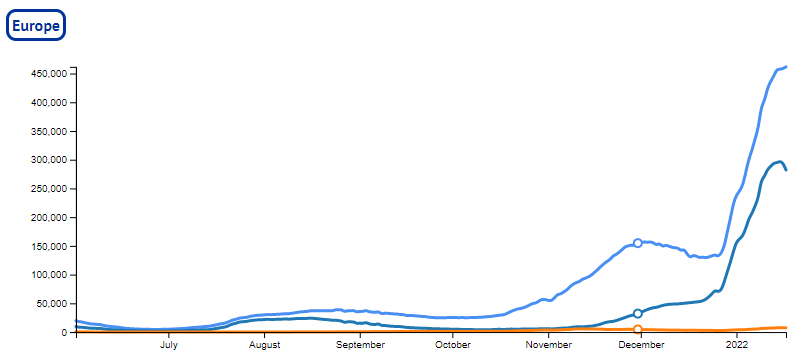
\includegraphics[width=1\linewidth]{img/line.png}
	\caption{Line Chart} \label{Fig4}}
\end{figure}

\subsection{Bar chart}
A bar chart is a chart or graph that presents categorical data with rectangular bars with heights or lengths proportional 
to the values that they represent. Therefore, it is used to show comparisons among discrete categories. One axis of the chart 
shows the specific categories being compared, and the other axis represents a measured value \cite{barchart}.

In our platform we used a {\em stacked bar chart} with the aims to compare different values and different countries at the same time. 
It shows the following data:
\begin{itemize}
	\item {\em Cases view}: It shows the percentage of positives over population in comparison with the percentage of deaths over population and with the stringency index. The purpose of this plot is to have a clear idea of how the stringency index of a nations influences the cases and the deaths.
	\item {\em Deaths view}: It shows the percentage of positives over population in comparison with the percentage of deaths over population and with the percentage of deaths over positives. The purpose of this plot is to have a focus on the deaths with respect the cases.
	\item {\em Vaccinations view}: It shows the percentages of vaccinated with one, two and three doses of vaccine.
\end{itemize}

Note that the data showed are related to the date selected as the end of the interval of time, so they are data of one day. Obviously this date can be changed.

Interactions:
\begin{itemize}
	\item {\em On mouse over}: It shows a tooltip with the data showed.
	\item {\em On Click}: It focus the countries selected. This event has effect also in all the other visualizations that will focus the selected country.
\end{itemize}

\begin{figure}
    \centering{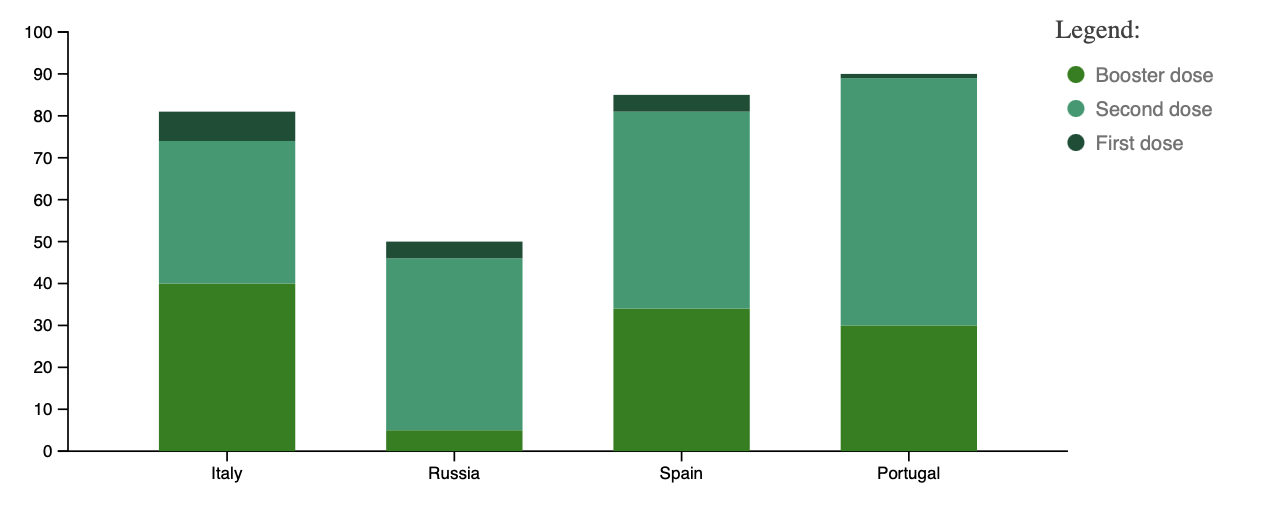
\includegraphics[width=1\linewidth]{img/bar.png}
	\caption{Bar Chart} \label{Fig5}}
\end{figure}

\subsection{PCA chart}
A scatter plot is a type of plot or mathematical
using Cartesian coordinates to display values for typically two variables for a set of data. If the points are coded (color/shape/size), 
one additional variable can be displayed. The data are displayed as a collection of points, each having the value of one variable 
determining the position on the horizontal axis and the value of the other variable determining the position on the vertical axis \cite{scatter}.

In EU CoVis-19 PCA chart shows the two principal components (2D visualization) of the data for each selected country. This chart is very useful because showing all the data for a country it makes possible to do comparison between 
countries and understand well that many nations have provided very few data, and as we have known for some time now, this is a factor that must be taken into account when comparing two or more countries about the covid pandemic.

PCA is also integrated as analytics, indeed it changes based on the countries selected.

Based on the views, the data taken in considerations is different:
\begin{itemize}
	\item {\em Cases and Deaths view}: ["new cases", "new cases smoothed", "total deaths", "new deaths", "new deaths smoothed", "stringency index"]
	\item {\em Vaccinations view}: ["new vaccinations smoothed", "people fully vaccinated", "people vaccinated", "total boosters"]
\end{itemize}

\begin{figure}
    \centering{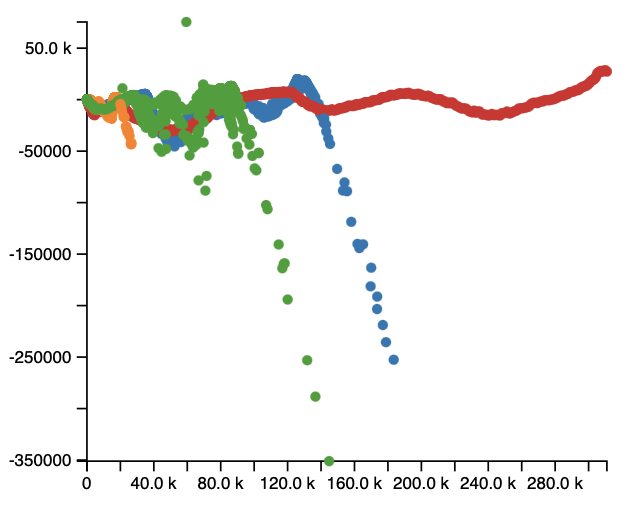
\includegraphics[width=0.7\linewidth]{img/pca.png} 
	\caption{PCA Chart} \label{Fig6}}
\end{figure}

\subsection{Parallel Coordinates chart}
Parallel plot or parallel coordinates plot allows to compare the feature of several individual observations (series) on a set of numeric variables. Each vertical bar represents a variable and often has its own scale. (The units can even be different). Values are then plotted as series of lines connected across each axis. \cite{paral}.

In our platform we used a {\em parallel coordinates chart} with the aims to compare different values of different countries at the same time. 
It shows the following data:
\begin{itemize}
	\item {\em Cases view}: ['Country', 'Population', 'Population density', 'Smokers', 'Cardiovasc death rate', 'Diabetes prevalence', 'Median Age']. 
	\item {\em Deaths and Vaccines views}: ['Country', 'Population', 'Population density', 'Life Expectancy', 'GDP pro capita', 'Human Development Index', 'Median Age']. 
\end{itemize}

In all three views we show the basic values that describe a nation, and which can be useful to better understand the pandemic numbers: Population, population density and median age. In addition, in the Cases views we wanted to give greater focus to factors (Smokers, Cardiovasc death rate and Diabetes prevalence) that could affect the respiratory tract and therefore cause a possible infection.

In Vaccines and Deaths views, on the other hand, we wanted to give greater relevance to three factors (Life Expectancy, Human Development Index and GDP per capita) which could be more easily attributable to causes of death or could highlight problems such as not being able to afford suitable treatments.

These factors also allow us to make a comparison based on the wealth of a particular nation.

\begin{figure}
    \centering{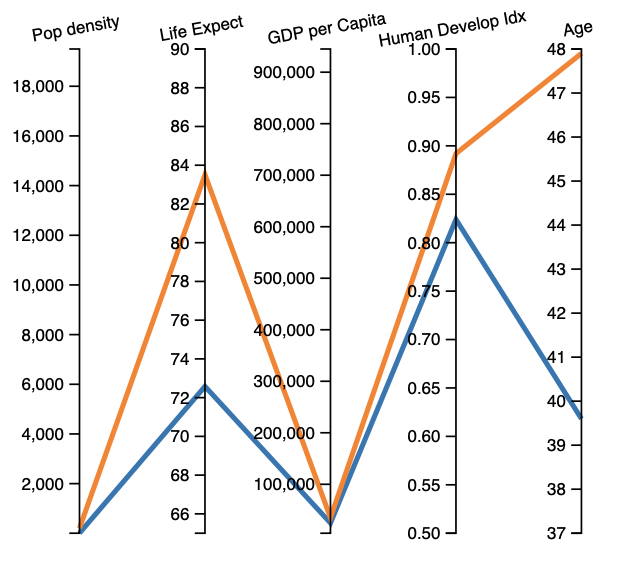
\includegraphics[width=0.7\linewidth]{img/paral.png} 
	\caption{Parallel Coordinates Chart} \label{Fig7}}
\end{figure}


\subsection{Table chart}
We have decided to use the table chart as a big legend for the current view. Indeed in the table are showed the names of the selected countries each of which with a color, that is the same color the nations have in all the other visualizations. With this choices we want simplify the views to the user and to make uniform the visualizations.
The table shows also the data presented in the parallel coordinates chart. The table is also interactive, so it has the ability to change the other visualizations.
Interactions:
\begin{itemize}
	\item {\em On Click}: It focus the countries selected. This event has effect also in all the other visualizations that will focus the selected country.
\end{itemize}

\begin{center}
    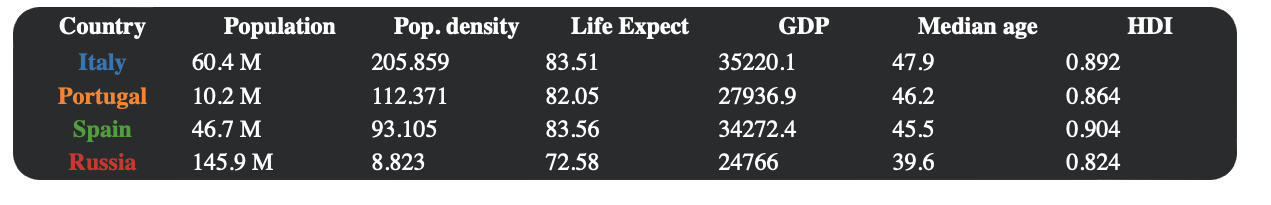
\includegraphics[width=1\linewidth]{img/table.png} 
\end{center}

\section{Analytics}
In our platform we will develop the following analytics:
\subsection{Simple: Comparisons, Aggregations and Operations} 
EU CoVis-19 has been designed and built to make the comparison between data from different European countries as simple as possible. All the data that are shown when one or more countries is selected from the map (or from the navbar) are the result of a computation that aggregates all the data of the selection and shows them in the various views.
So the aggregations are based on countries selected and interval of time (Date) and they are computed at the selection (Not precomputed). This means also that there are a very high number of possible combination of selections that a user could compute. 

About {\em Parallel Coordinates} and {\em TableChart} they simple aggregation, while in the {\em LineChart} we have an aggregation plus a summation of the data because to show the trend during the interval of time select we have to sum the data of every day. Furthermore, all the percentages shown in the {\em BarChart} are the result of a computation, and they are computed at the selection and not predefined.

{\em Europe data}, shown at the beginning or when the Europe button is clicked, are computed at the selection, they are the sum of all other countries present in the dataset.

\subsection{Complex: PCA}
In this project we have decided not to use Principal Component analysis only as a dimensionality reduction of the dataset, and to show all the data, but also in this case we have tried to make sense of the platform by making the data shown by PCA useful for making comparisons. As already mentioned above, PCA is applied to different data based on the views chosen. This choice helps us to understand how much data we have of each country, because looking at the visualization we realize that some countries provide much more data than others (At least from the sources from which the dataset collects data). This can be a useful yardstick for not reaching hasty conclusions on the data of some countries. PCA is an analytics because the computation is done at each selection and is not precomputed. It is an expensive computation made up of several steps, which is why for us it is a complex analytics.


\begin{figure*}[!t]
	\centering{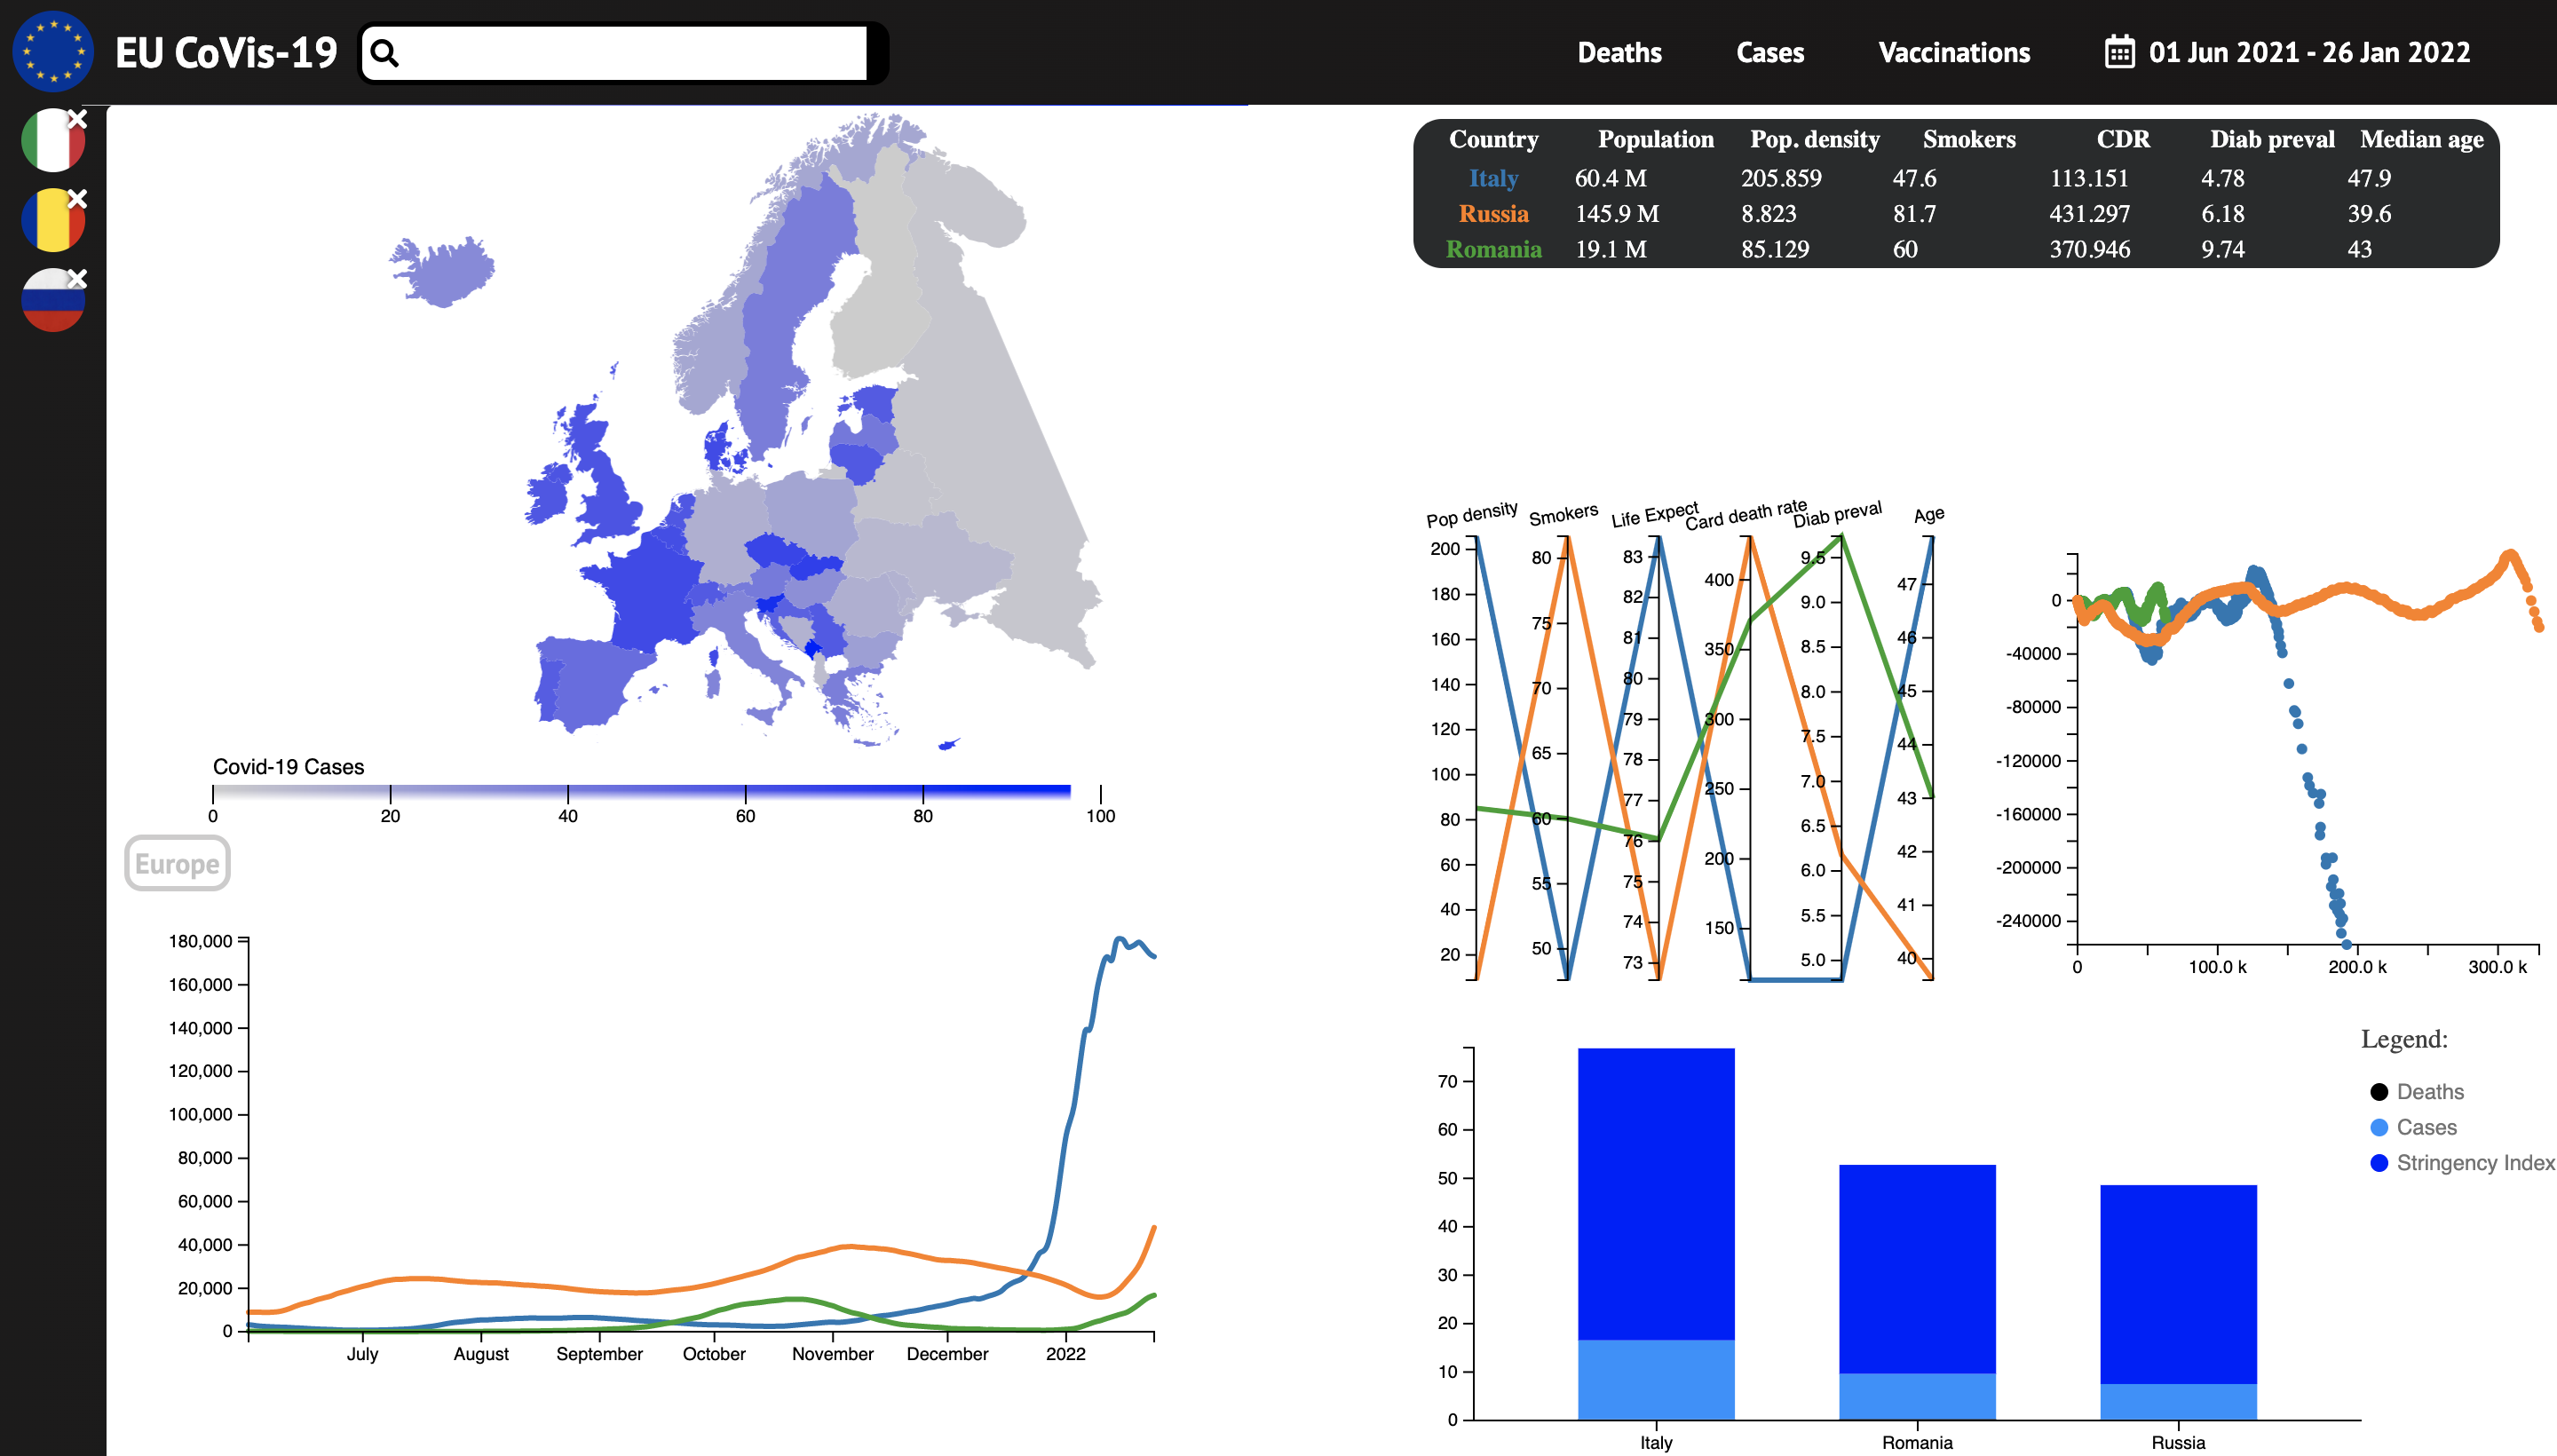
\includegraphics[width=1\linewidth]{img/fig1.png}
	\caption{Cases view} \label{Fig1}}
\end{figure*}
	
\begin{figure*}[!t]
	\centering{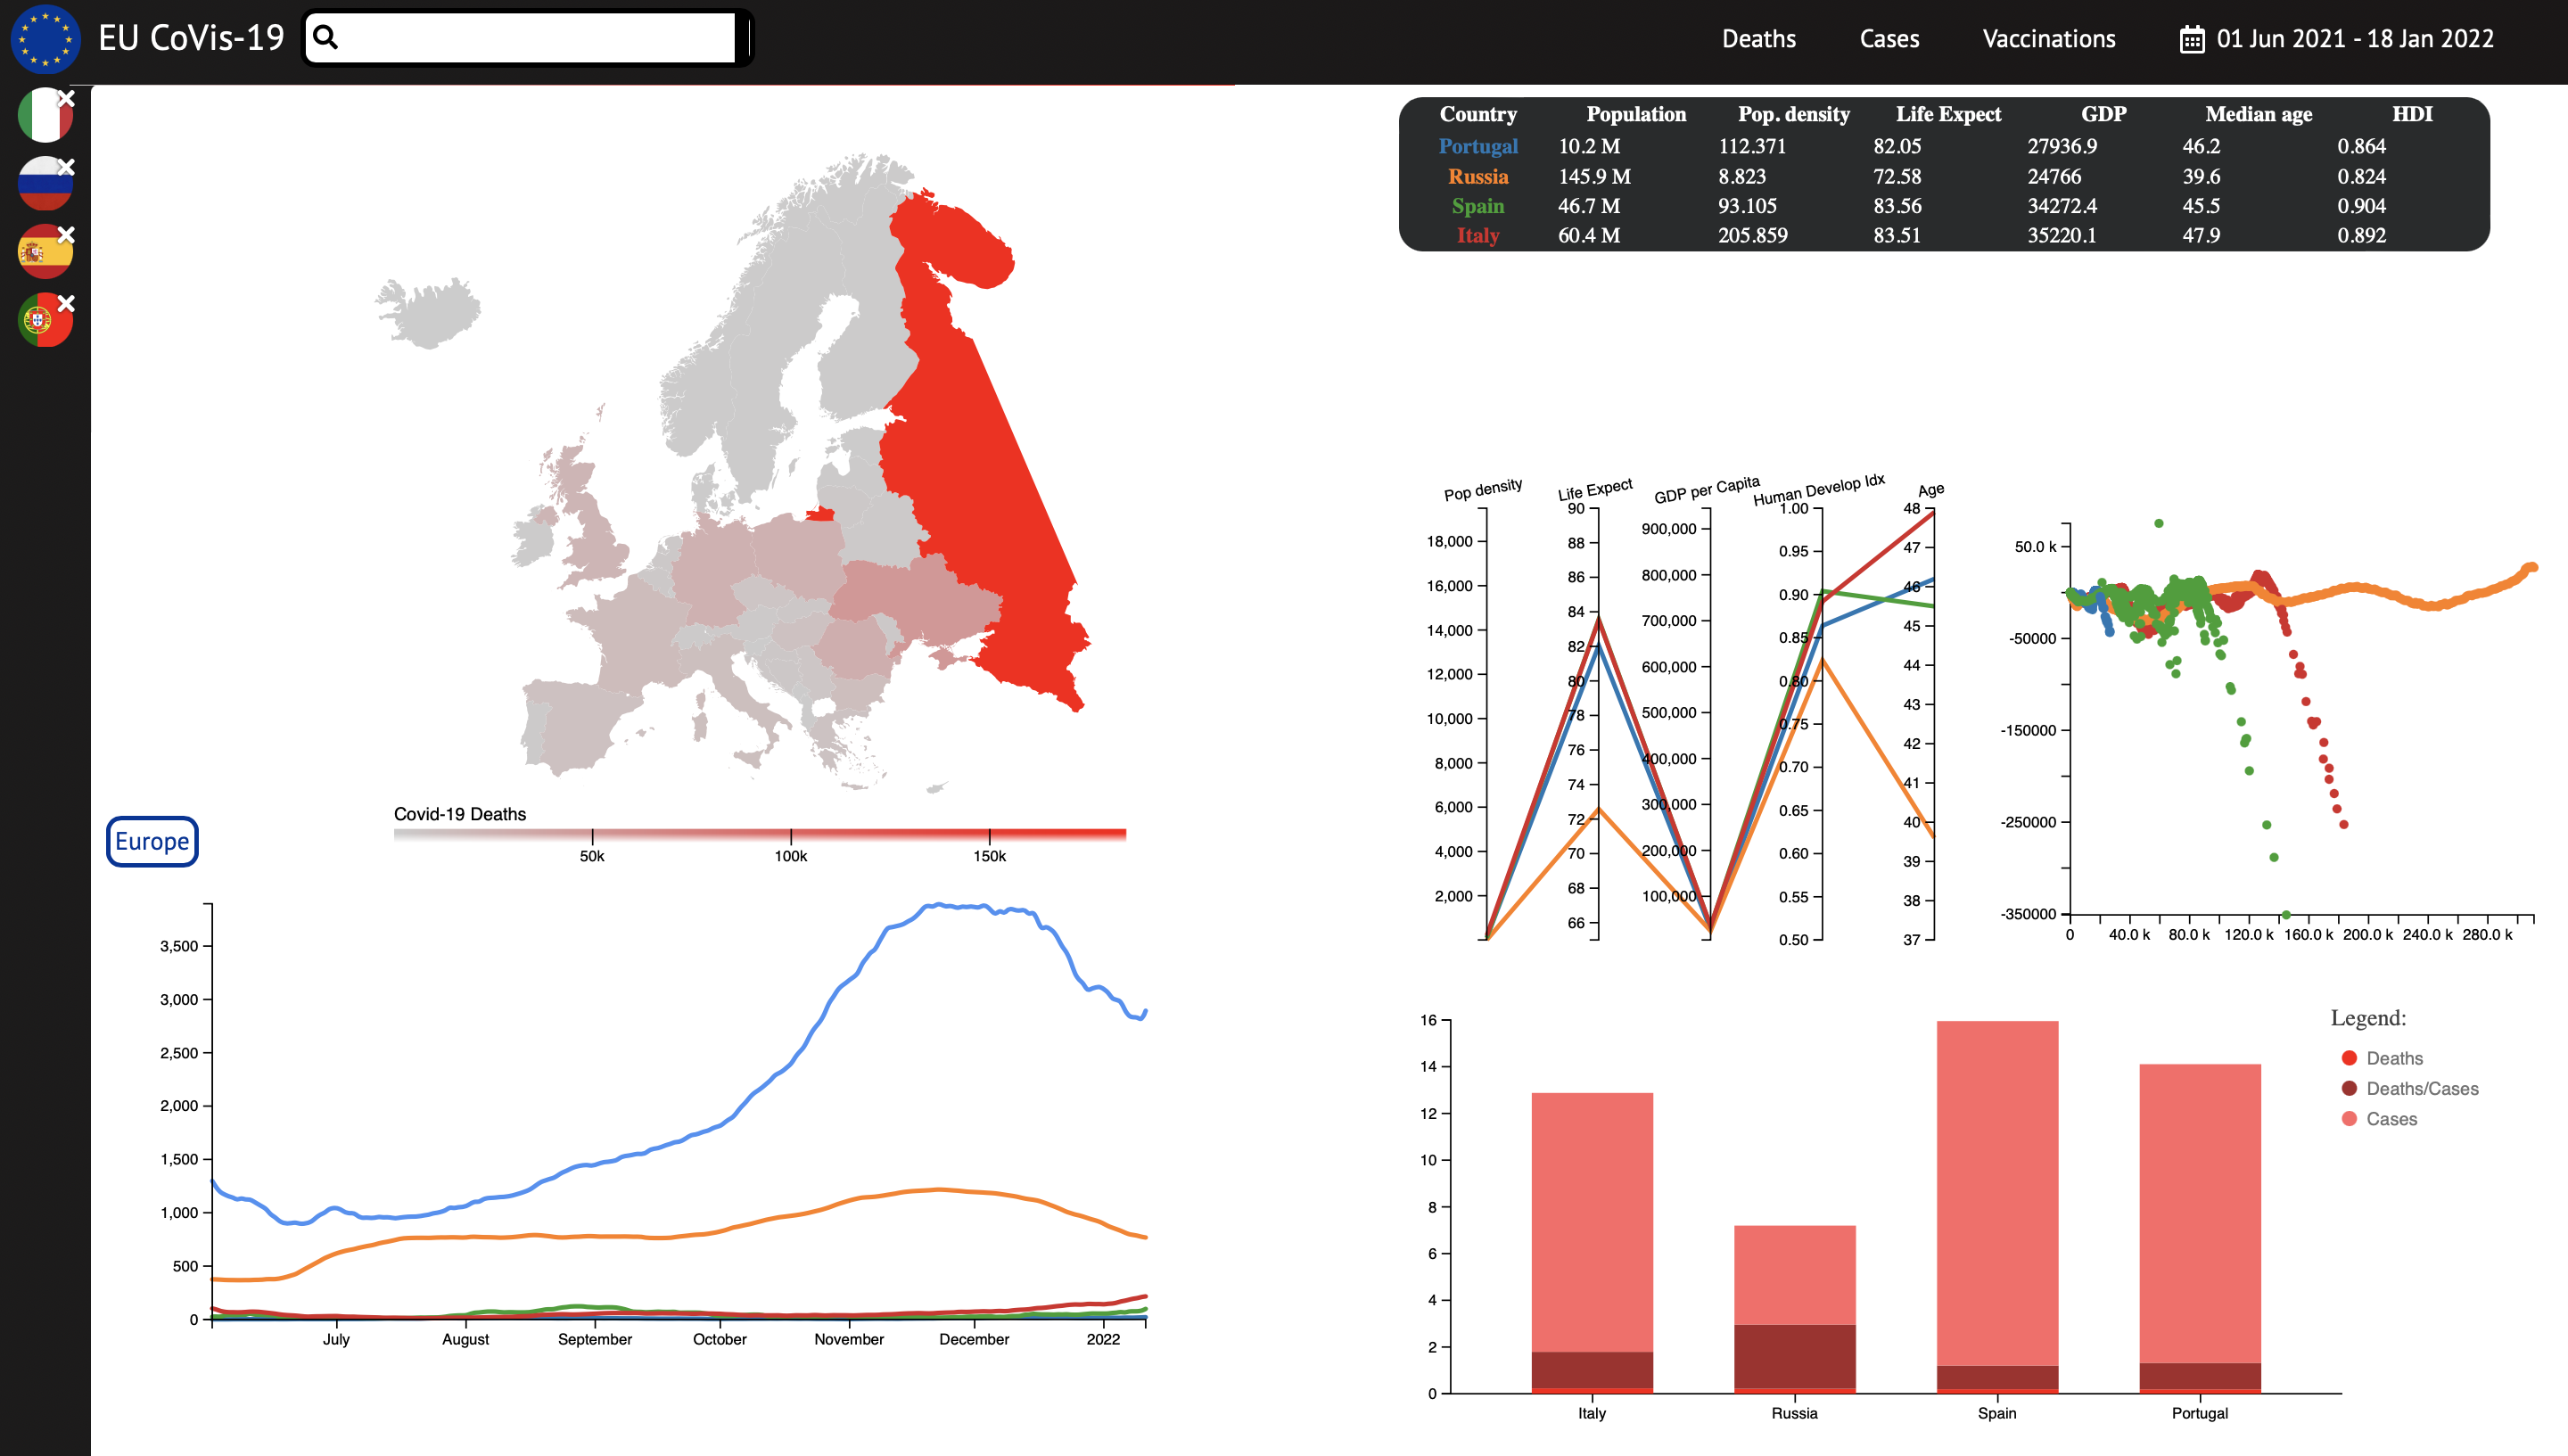
\includegraphics[width=1\linewidth]{img/fig2.png}
	\caption{Deaths view} \label{Fig2}}
\end{figure*}

\begin{figure*}[!t]
	\centering{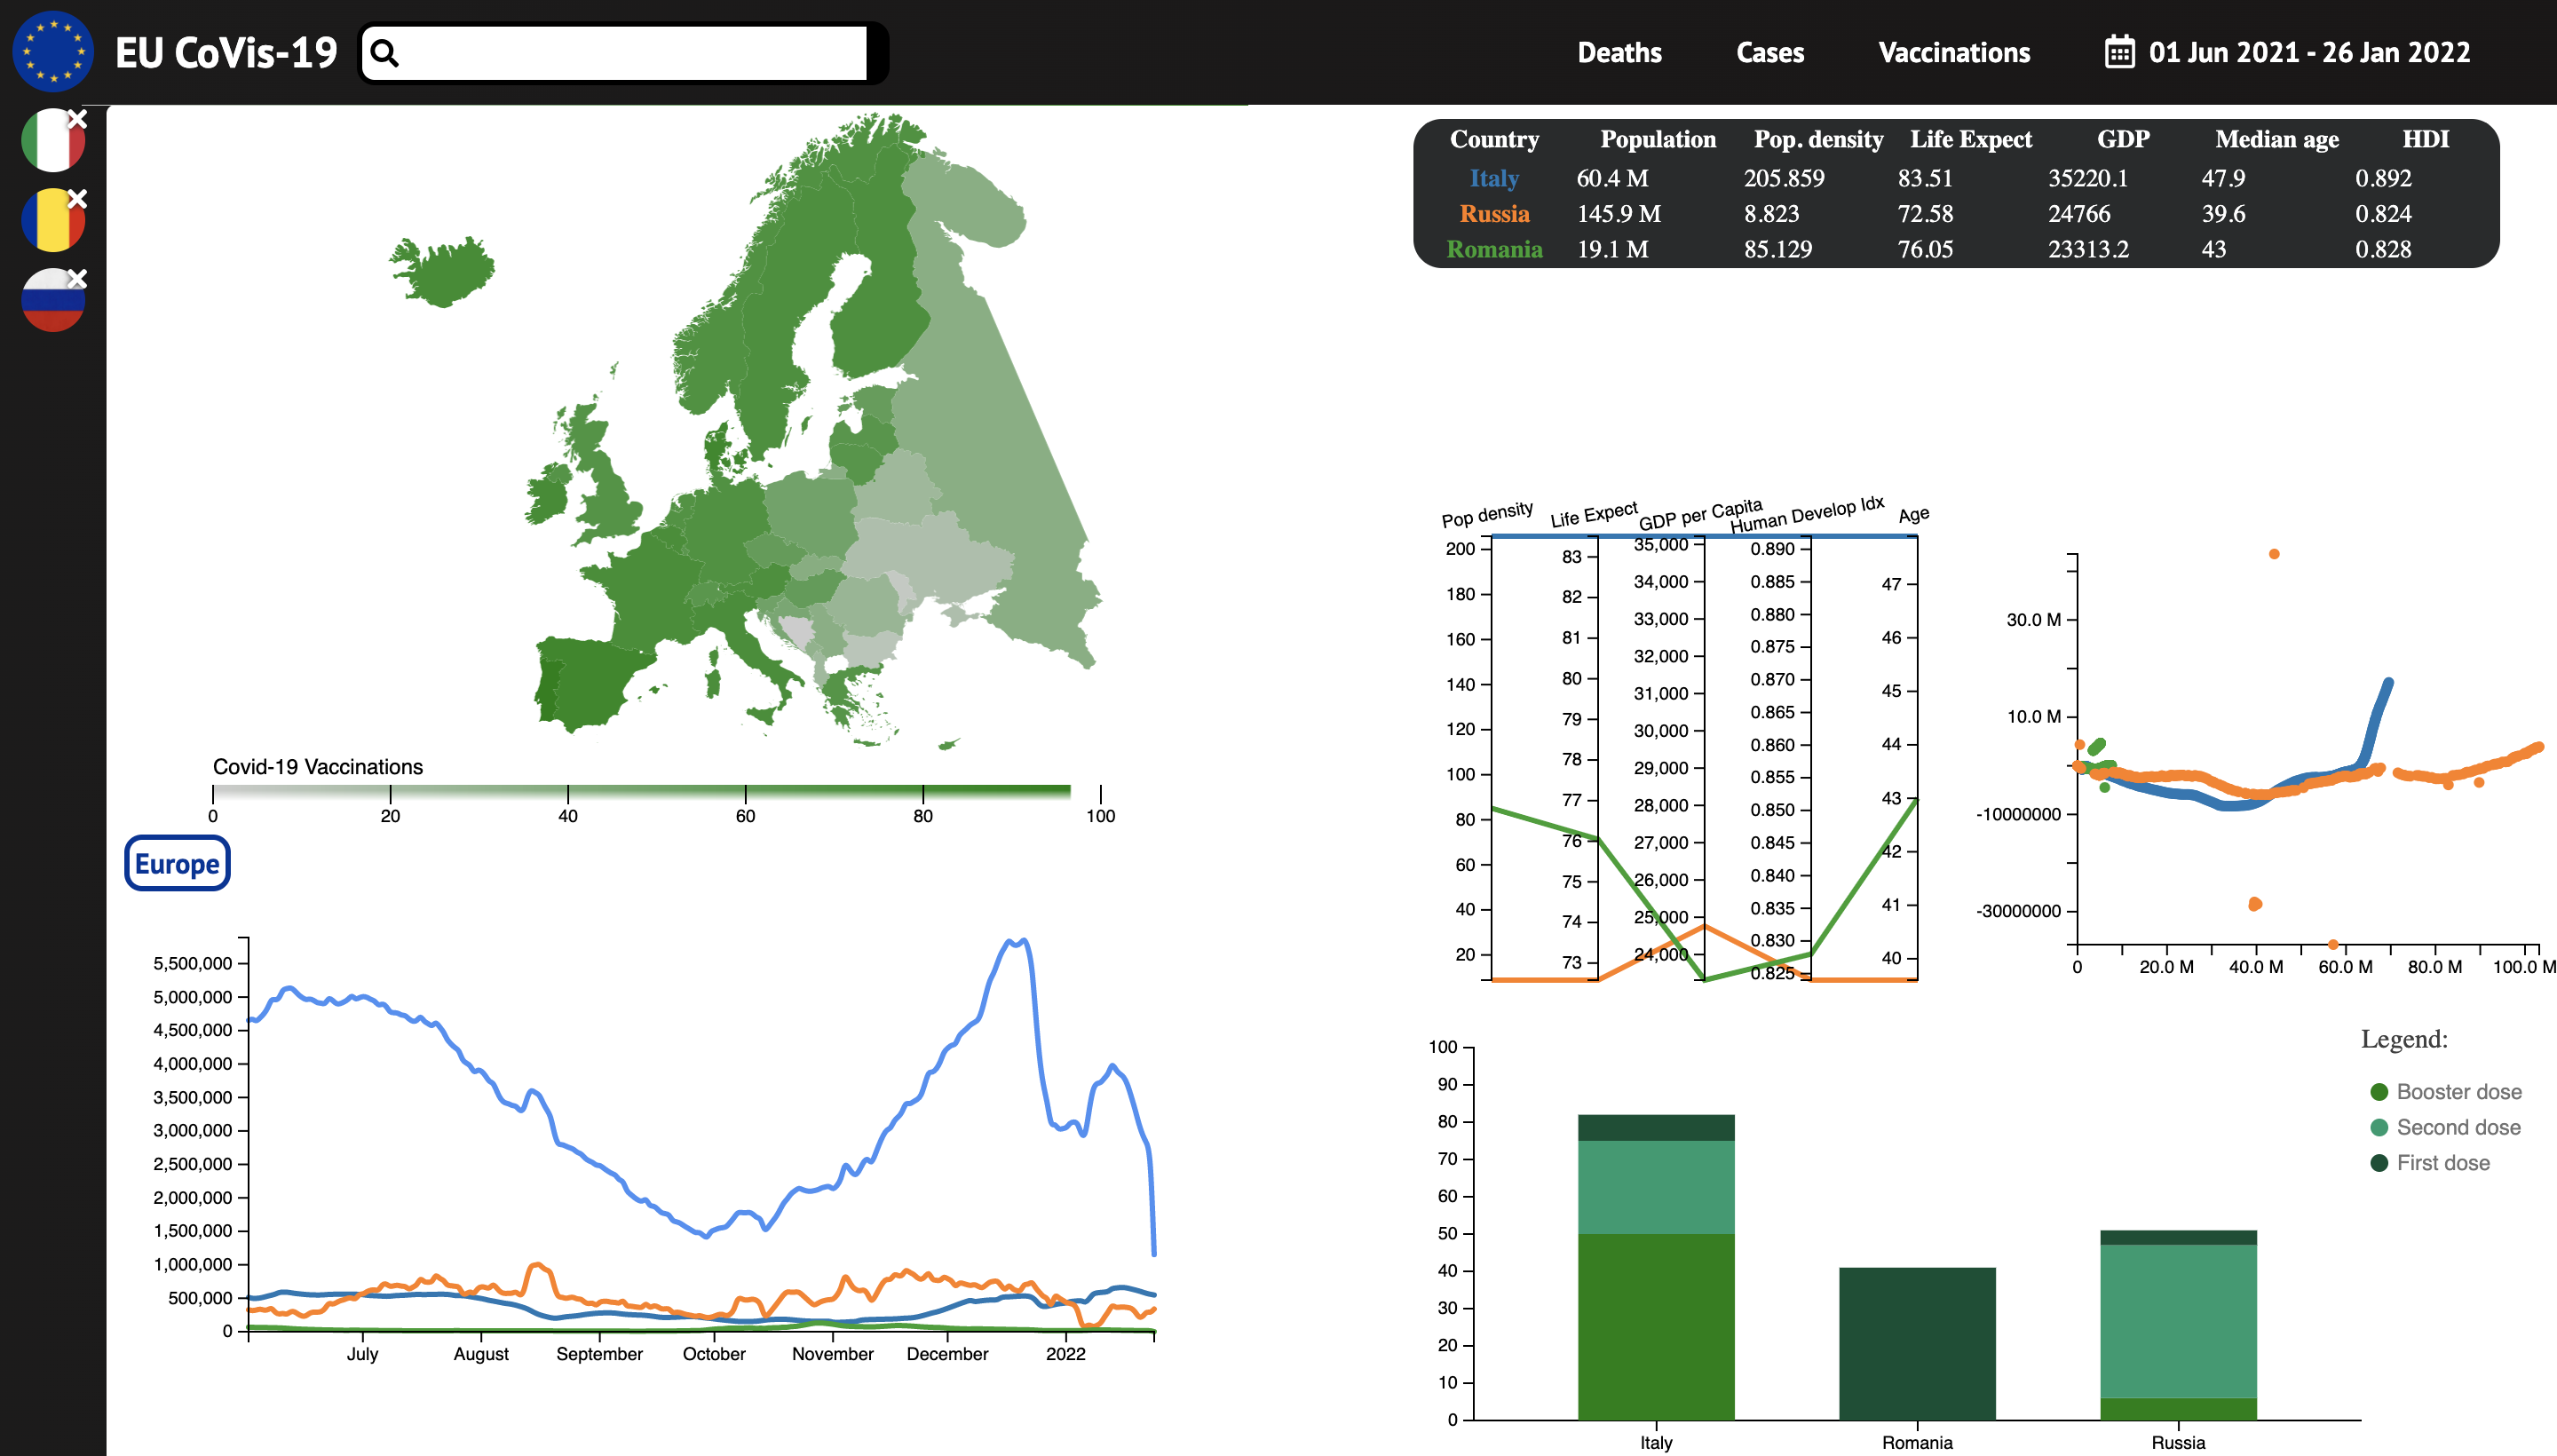
\includegraphics[width=1\linewidth]{img/fig3.png}
	\caption{Vaccinations view} \label{Fig3}}
\end{figure*}


\section{Case of study}

\section{Conclusion and Future Work}
Over the past year, there has been work to visualize and analyze different aspects of big data related to COVID-19. However, most existing viewers focus on visualizing temporal and / or spatial trends, case numbers and mortality, but none take into account all the other possible factors that can affect a nation's pandemic picture. Plus it is very difficult for viewers to make comparisons across multiple views since almost all of them are multi-page and not one-page structured. In this project, we focus on the already existing factors of the various countries and make the comparison of the data as efficient as possible. Our key contributions include the design and development of a big data visualization and visual analysis tool for epidemiological data of COVID-19. By incorporating PCAs as analytics we also provide a tool that helps to ideally understand how different country data is and how much data is being provided. We give users the flexibility to make as many comparisons as they want. The results of the visualizations can help researchers, politicians, but also ordinary people to gain a better understanding of COVID-19 and thus enable them to fight the disease.

Our tool can be applicable to other real-world applications, by changing the data in the dataset, having such a broad view of an issue can help combat it. As a work in progress and in the future, we explore the possibility of incorporating other tools into the project, with particular reference to machine learning techniques that can make predictions on trends or help to better understand the data in possession.


\begin{thebibliography}{00}

\bibitem{dataset} https://github.com/owid/covid-19-data
\bibitem{dimRed} https://en.wikipedia.org/wiki/Dimensionality\_reduction

\bibitem{javascript} https://www.javascript.com/
\bibitem{node} https://nodejs.org/it/
\bibitem{mongo} https://www.mongodb.com
\bibitem{d3} https://d3js.org/
\bibitem{map} https://en.wikipedia.org/wiki/Choropleth\_map
\bibitem{barchart} https://en.wikipedia.org/wiki/Bar\_chart
\bibitem{scatter} https://en.wikipedia.org/wiki/Scatter\_plot
\bibitem{paral} https://www.data-to-viz.com/graph/parallel.html
\bibitem{line} https://en.wikipedia.org/wiki/Line\_chart
\bibitem{vis1} P. Le Bras, et al., “Visualising COVID-19 research,” 2020, CoRR abs/2005.06380
\bibitem{vis2} J. Tu, M. Verhagen, B. Cochran, J. Pustejovsky, “Exploration and discovery of the COVID-19 literature through semantic visualization,” 2020, CoRR abs/2007.01800
\bibitem{vis3} F. Wolinski, “Visualization of diseases at risk in the COVID-19 literature,” 2020, CoRR abs/2005.00848
\bibitem{vis4} F. Zuo, et al., “An interactive data visualization and analytics tool to evaluate mobility and sociability trends during COVID-19,” in ACM KDD Workship on UrbComp 2020, pp. 5:1-5:5
\bibitem{vis5} S. Zhang, Y. Cai, J. Li, “Visualization of COVID-19 spread based on spread and extinction indexes,” Sci. China Inf. Sci. 63(6), 2020, pp. 164102:1-164102:3
\bibitem{vis6} WorldHealthOrganization(WHO),WHOcoronavirusdisease(COVID- 19) dashboard. https://covid19.who.int/
\bibitem{vis7} (CSSE) at Johns Hopkins University (JHU) https://coronavirus.jhu.edu/map.html
\bibitem{vis8} European Center for Disease Prevention and Control https://www.ecdc.europa.eu/en/covid-19
\bibitem{vis9} Our World in Data, Coronavirus Pandemic (COVID-19): https://ourworldindata.org/coronavirus 

\end{thebibliography}
\end{document}